\begin{tikzpicture}
  \foreach \x/\c in {0/orange!70, 2/gray!40, 4/orange!70} {
    \draw[fill=\c] (\x,0) rectangle (\x+2,4.9);
    \foreach \y in {0.7,1.4,...,4.2} {
      \draw (\x,\y) -- (\x+2,\y);
    }
  }
  \draw[thick] (0,-0.15) -- (0,-0.35);
  \draw[thick] (2,-0.15) -- (2,-0.35);
  \draw[thick] (4,-0.15) -- (4,-0.35);
  \draw[thick] (6,-0.15) -- (6,-0.35);
  \draw[<->] (0,-0.25) -- (2,-0.25);
  \node at (1,-0.55) {$\dfrac{d}{3}$};
  \draw[<->] (2,-0.25) -- (4,-0.25);
  \node at (3,-0.55) {$\dfrac{d}{3}$};
  \draw[<->] (4,-0.25) -- (6,-0.25);
  \node at (5,-0.55) {$\dfrac{d}{3}$};
\end{tikzpicture}
